% Indicate the main file. Must go at the beginning of the file.
% !TEX root = ../main.tex

%----------------------------------------------------------------------------------------
% CHAPTER TEMPLATE
%----------------------------------------------------------------------------------------


\chapter{Disseny del front end} % Main chapter title

\label{Disseny del front end} % Change X to a consecutive number; for referencing this chapter elsewhere, use \ref{ChapterX}

%----------------------------------------------------------------------------------------
% SECCIÓ 1: Disseny del front end
%----------------------------------------------------------------------------------------
Aquest treball no se centra en el desenvolupament d'una aplicació o producte i el front end s'ha fet per presentar un treball complet i per facilitar l'anàlisi i generació de les instàncies. Als següents apartats es fa una explicació de com s'ha dissenyat aquesta part del treball sense entrar molt en detall, ja que aquest no és l'enfocament principal del projecte.

\section{Distribució de la pàgina web}
Com s'ha explicat per fer la interfície d'usuari s'ha optat per fer-la en una web. Aquesta està distribuïda en tres parts:
\subsection{Pàgina principal}
La pàgina principal és on es rep l'usuari, aquesta conté una breu descripció del projecte i com usar la web. A més també inclou un menú a la dreta amb el qual es pot navegar als dos apartats principals, la generació d'instàncies i la visualització d'instàncies.\\

\begin{figure}[H]
    \centering
    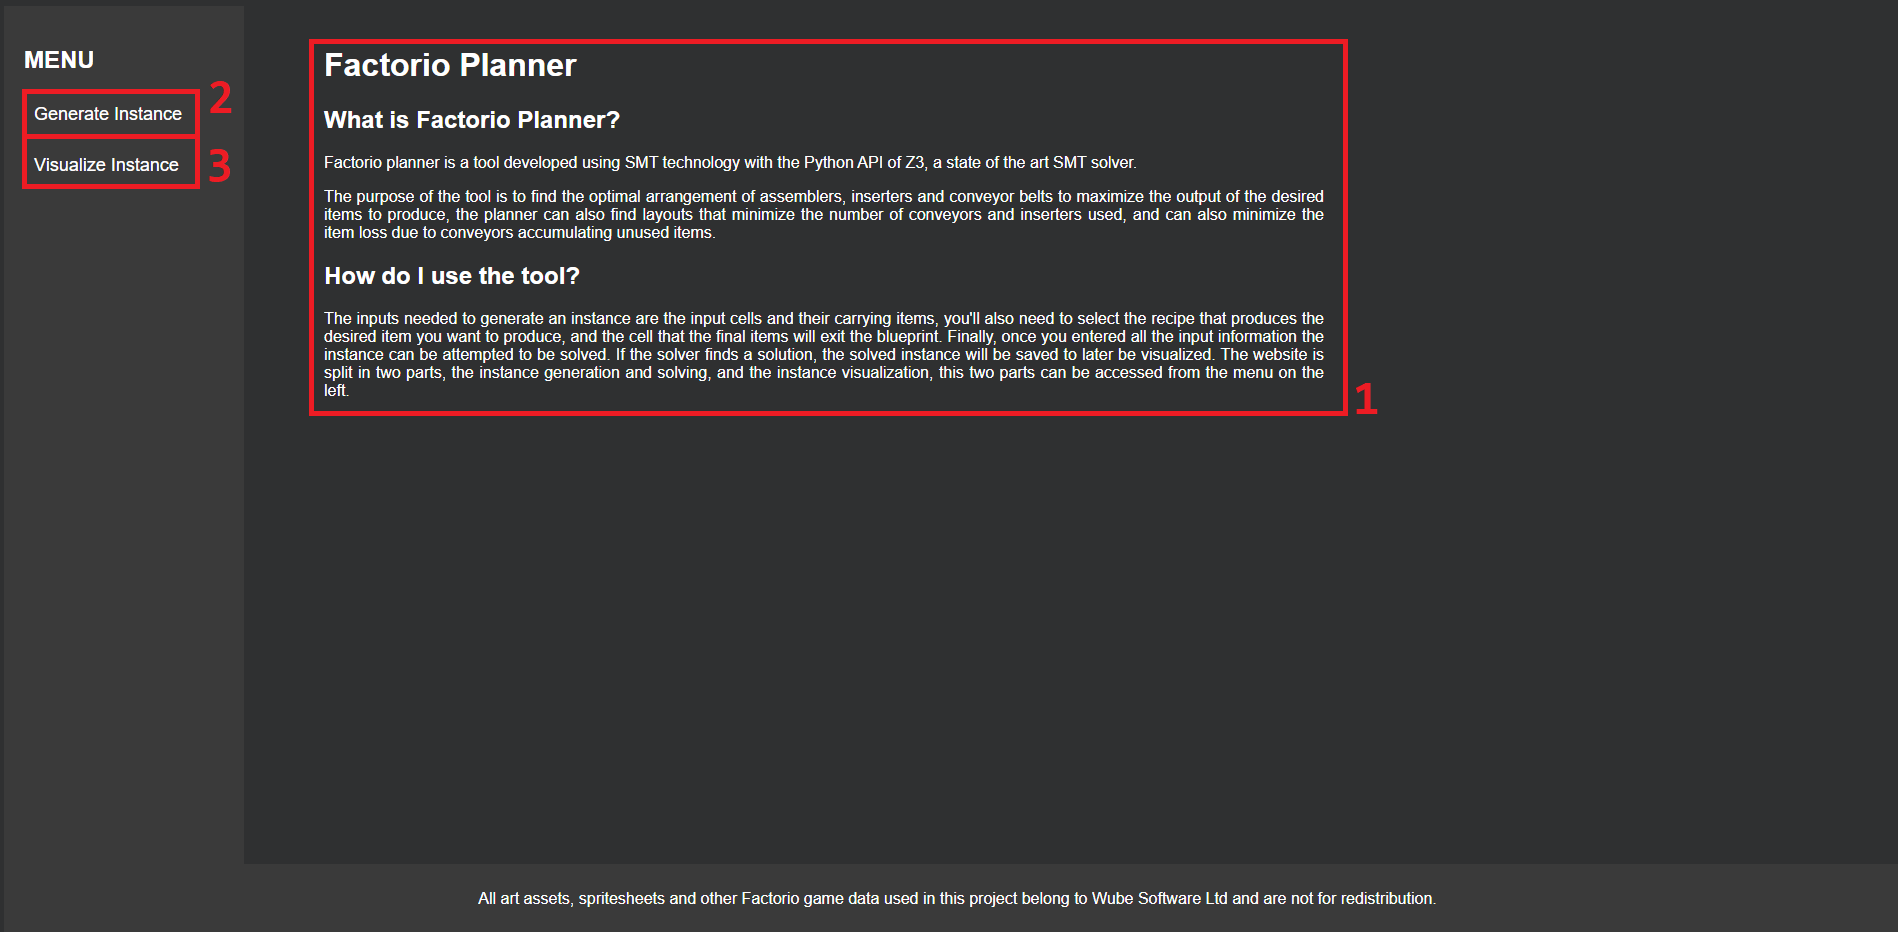
\includegraphics[width=1\linewidth]{Figures//captures_web/home_web.png}
    \caption{Plana principal de la web (1.Descripció de la web, 2.Opció del menú per generar instàncies, 3.Opció del menú per visualitzar instàncies)}
    \label{fig:home-webpage}
\end{figure}

\subsection{Generar instàncies}\label{subsec:generar-instancies}
Una de les funcionalitats principals de la interfície és poder generar instàncies de manera automàtica. Aquesta funcionalitat es troba a l'apartat \textit{Generate Instance} de la pàgina web. Des d'aquí sobre una pàgina nova la qual està separada en 4 seccions. Les tres primeres seccions són per afegir la informació d'entrada pel model:

\subsubsection{Objecte a produir}
En aquest apartat s'ha de seleccionar l'arxiu on es guarden totes les receptes del joc, concretament es troba al directori \texttt{/recipes} del projecte. Amb l'arxiu carregat es pot seleccionar l'objecte que es vol produir i a la web es carrega quins objectes es necessiten per fabricar-lo i en cas que l'objecte depengui de més receptes aquestes es mostraran juntament amb els objectes addicionals requerits per produir-los. D'aquesta manera és molt còmode saber els objectes i receptes implicats.
\begin{figure}[H]
    \centering
    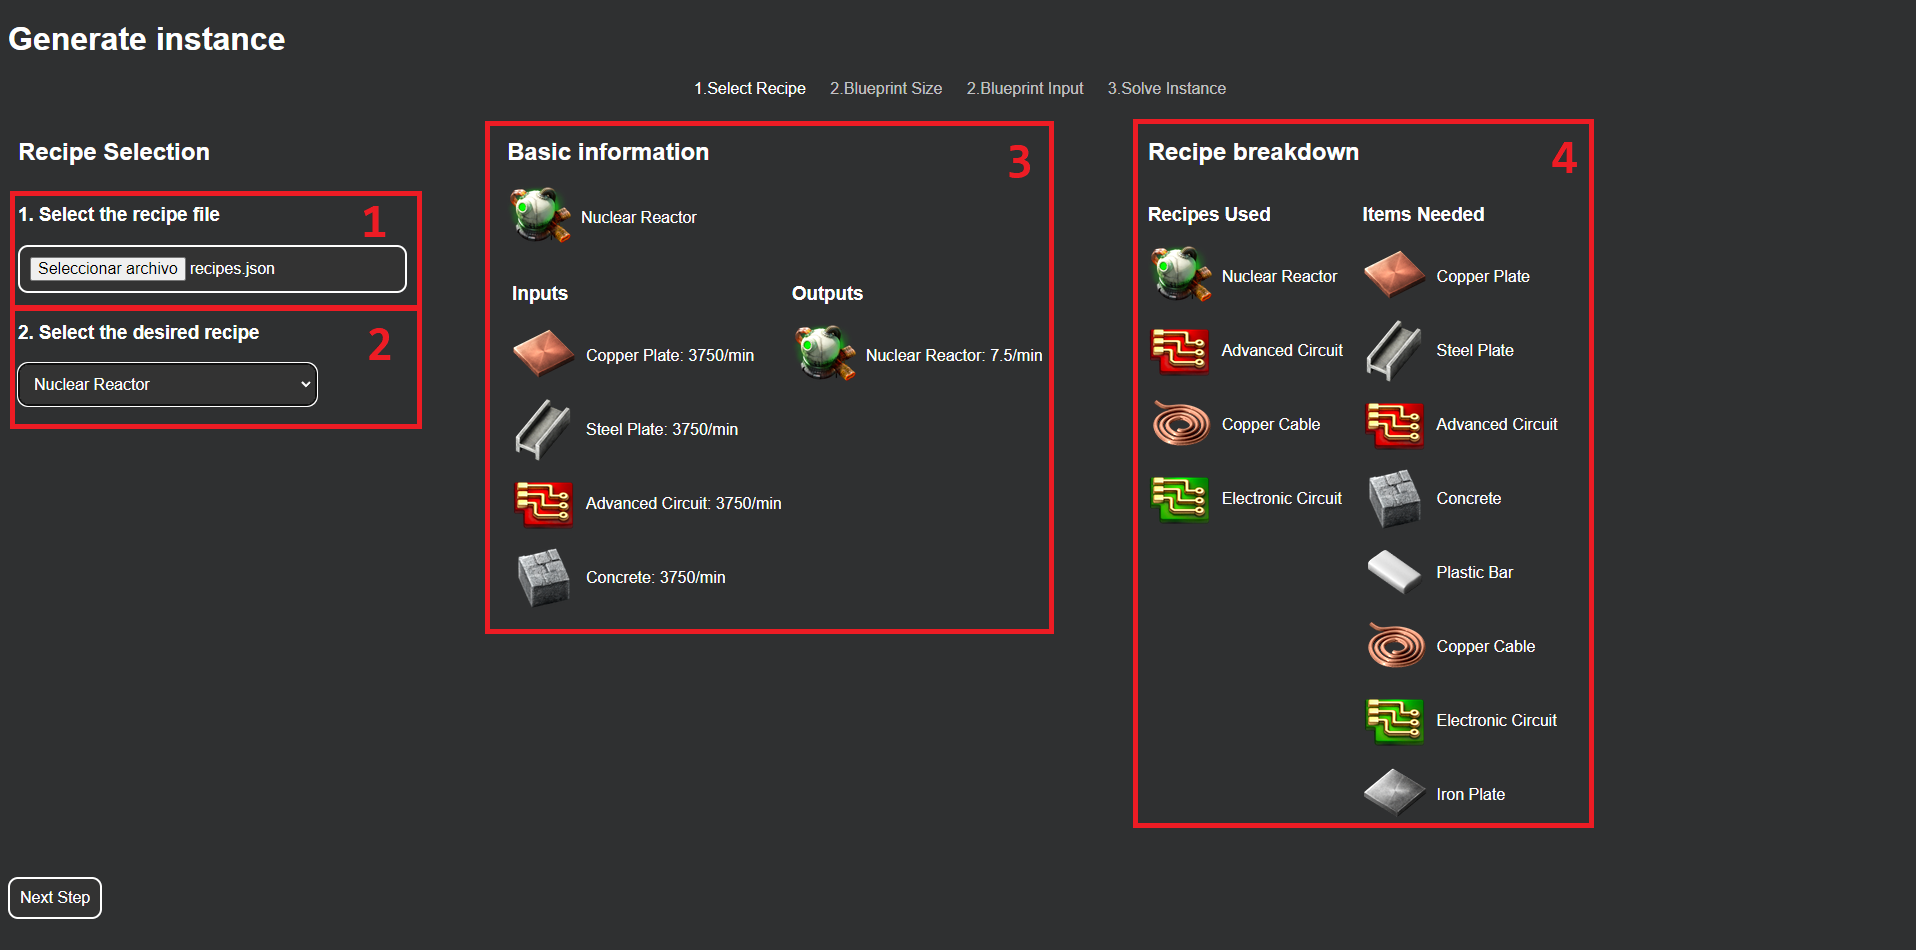
\includegraphics[width=1\linewidth]{Figures//captures_web/generate_instance_recipe_web.png}
    \caption{Primera part de la generació d'una instància (1.Seleccionar arxiu amb les receptes, 2.Seleccionar objecte a produir, 3.Informació de la recepta que produeix l'objecte), 4.Receptes implicades en la producció de l'objecte els objectes implicats)}
    \label{fig:generate_instance_recipe}
\end{figure}

\subsubsection{Mida del blueprint}
Aquest apartat és molt simple, només tracta de dos inputs d'HTML on s'han d'entrar les dimensions del blueprint.
\begin{figure}[H]
    \centering
    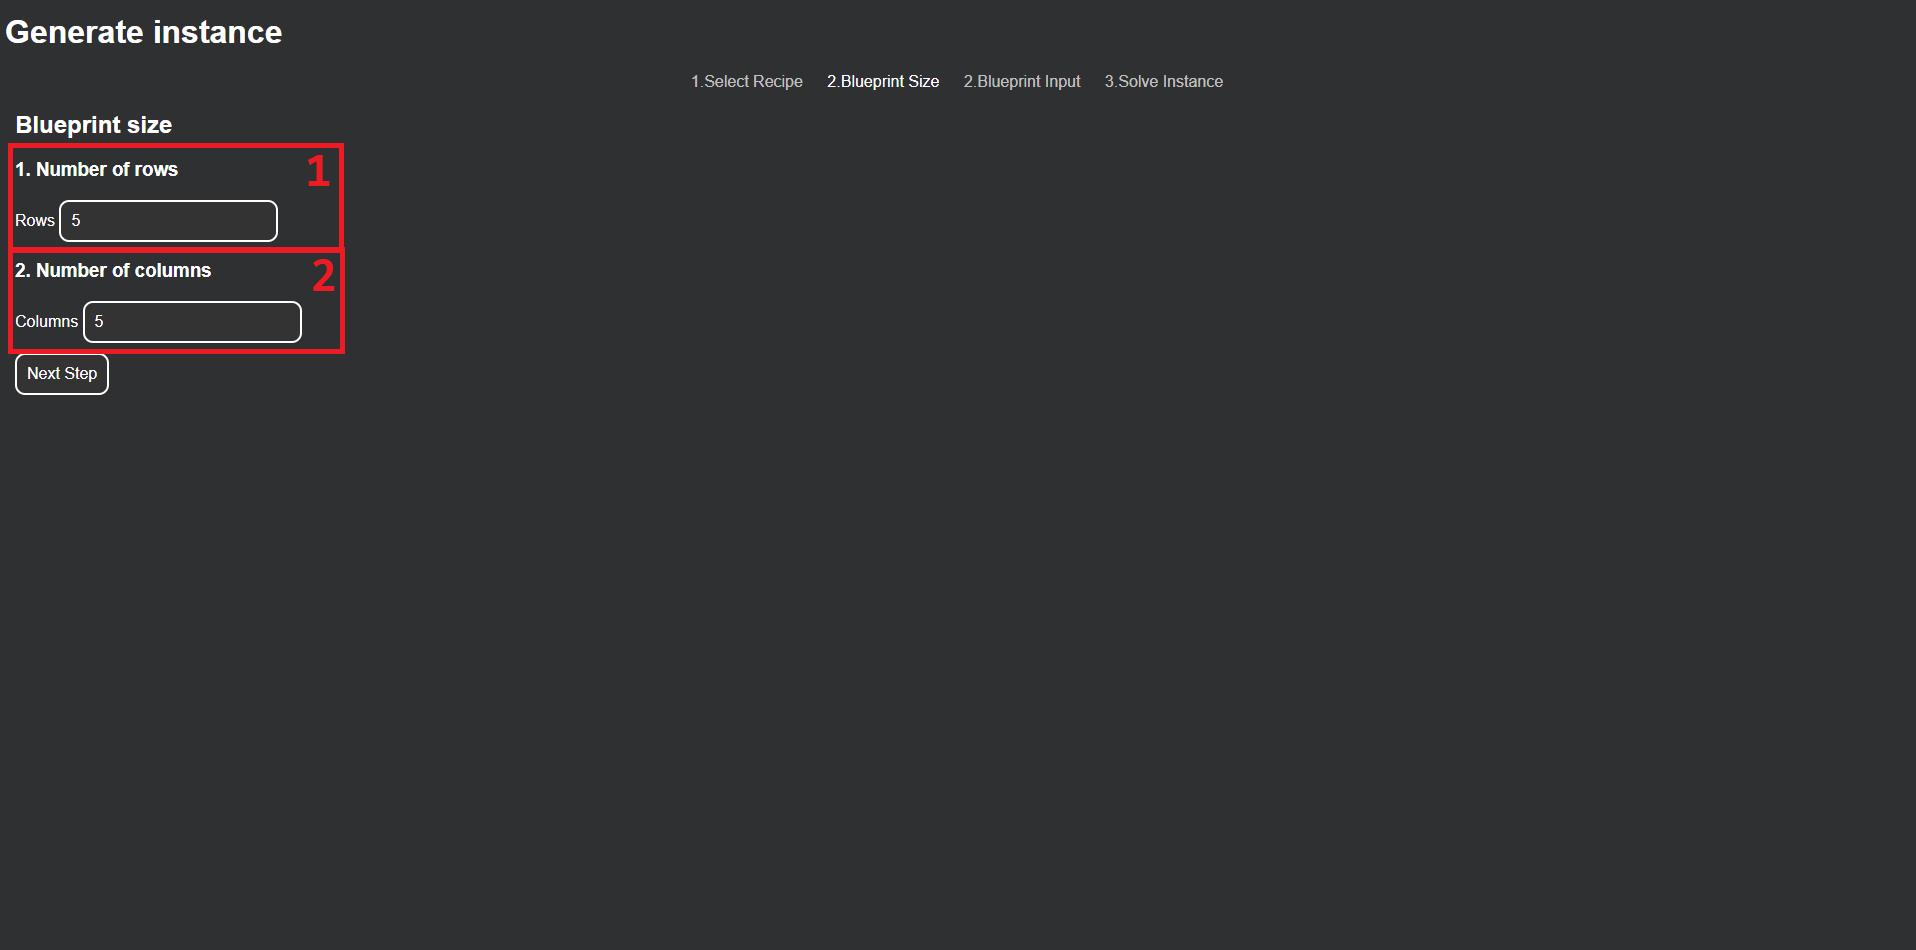
\includegraphics[width=1\linewidth]{Figures//captures_web/generate_instance_size_web.png}
    \caption{Plana web amb el pas 2 on s'ha de seleccionar la mida del blueprint (1.Seleccionar el nombre de files, 2.Seleccionar el nombre de columnes)}
    \label{fig:generate_instance_size}
\end{figure}

\subsubsection{Entrades i sortides del blueprint}
La selecció de quines caselles són d'entrada i sortida i el tipus objectes que han de transportar, és una de les parts més importants de les entrades del model i també una de les més complexes d'implementar, ja que implica poder clicar en una graella, seleccionar l'objecte i determinar si és una casella d'entrada i sortida, tot això mantenint una retroacció visual per saber el que s'està fent.\\

El funcionament és el següent, en funció de la mida entrada a la secció anterior i la recepta seleccionada al primer apartat del generador d'instàncies, aquesta part conté una graella interactiva on podem fer clic esquerre sobre les caselles i a la dreta de la graella apareixerà la informació relativa a la casella. Aquesta informació ens diu quin objecte conté el qual es pot seleccionar en un desplegable que contindrà els objectes que es necessiten per produir l'objecte objectiu, a més també ens diu si la casella és d'entrada o sortida.\\
Quan se seleccioni un objecte aquest es mostra a la graella de forma visual juntament amb un punt verd que indica que la casella és d'entrada. En cas que se seleccioni com a casella de sortida, es mostra un punt vermell.

\begin{figure}[H]
    \centering
    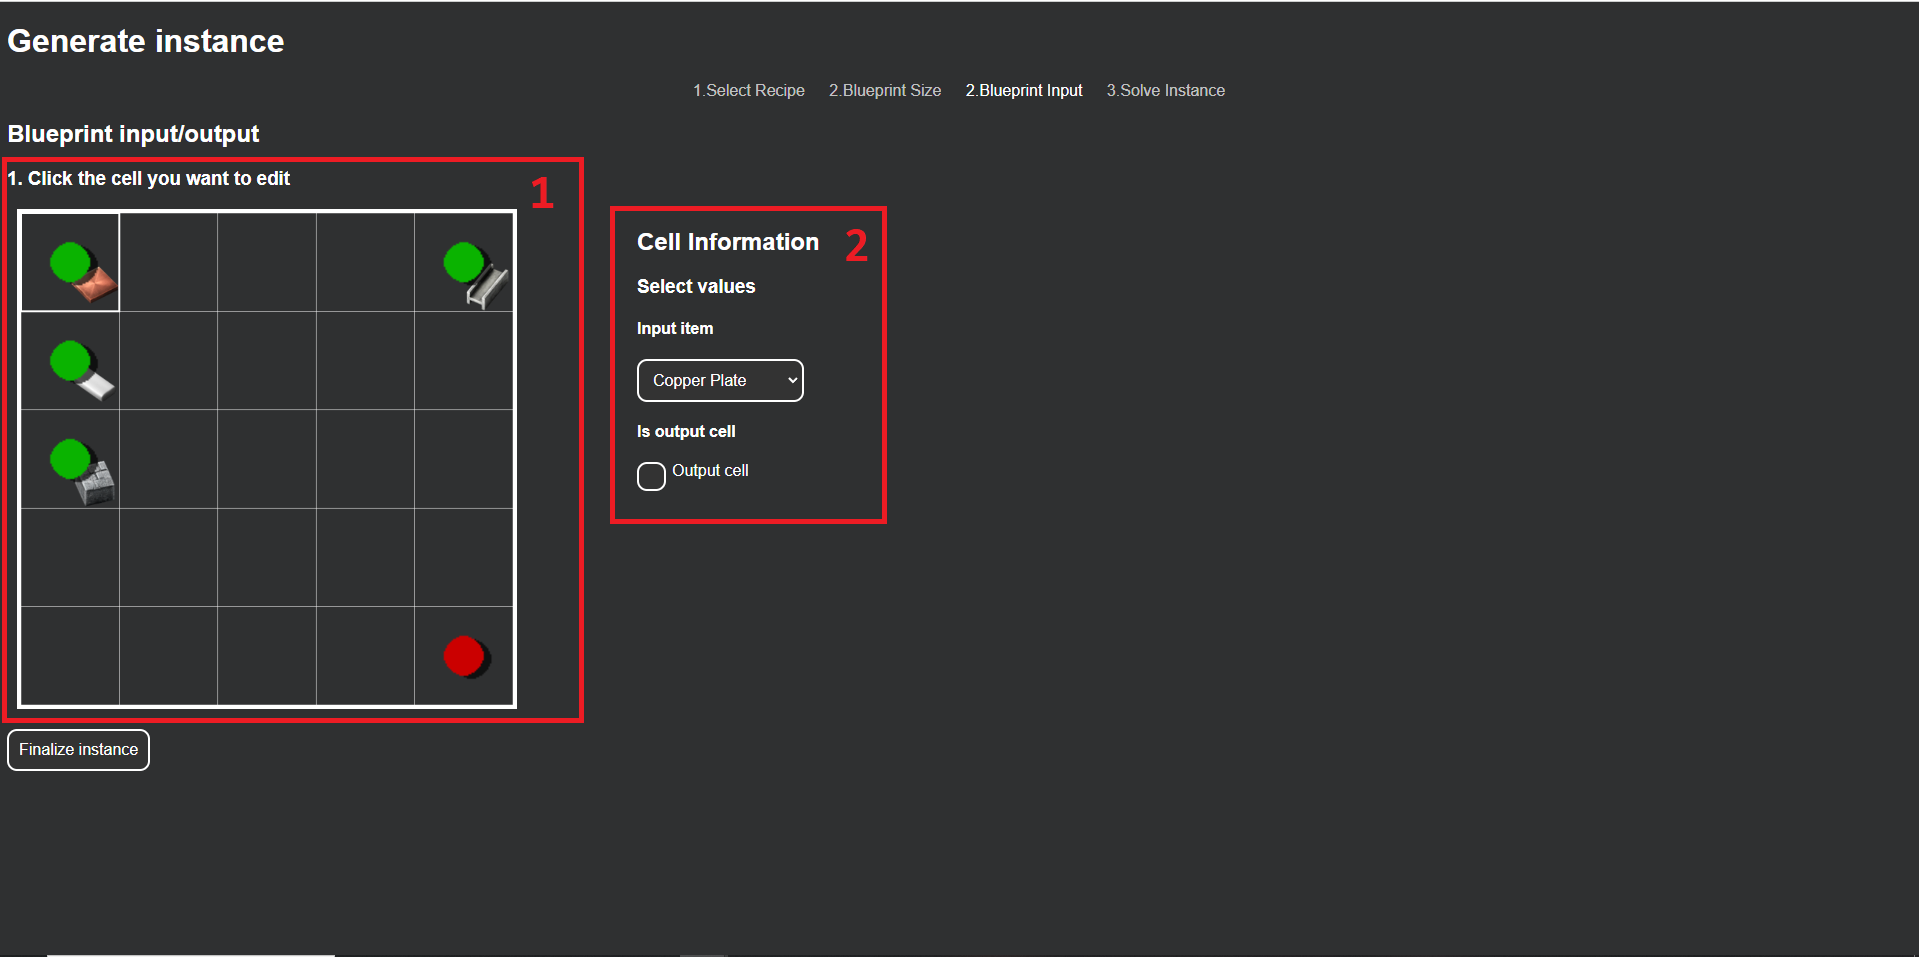
\includegraphics[width=1\linewidth]{Figures//captures_web/generate_instance_input_web.png}
    \caption{Plana web amb el pas 3 on s'han de seleccionar les entrades i sortides del blueprint (1.Graella interactiva, 2.Informació de la casella seleccionada)}
    \label{fig:generate_instance_input}
\end{figure}

\subsubsection{Resoldre la instància}
L'últim pas del procés de la generació de la instància tracta de seleccionar el criteri d'optimització i enviar la instància al back-end perquè sigui solucionada. Si la instància és resolta, s'informa el temps que tarda i l'estat (SAT, UNSAT o TIMED OUT), tot seguit es pot clicar el botó de descarregar la instància resolta per ser visualitzada a l'apartat de la web del visualitzador d'instàncies.
\begin{figure}[H]
    \centering
    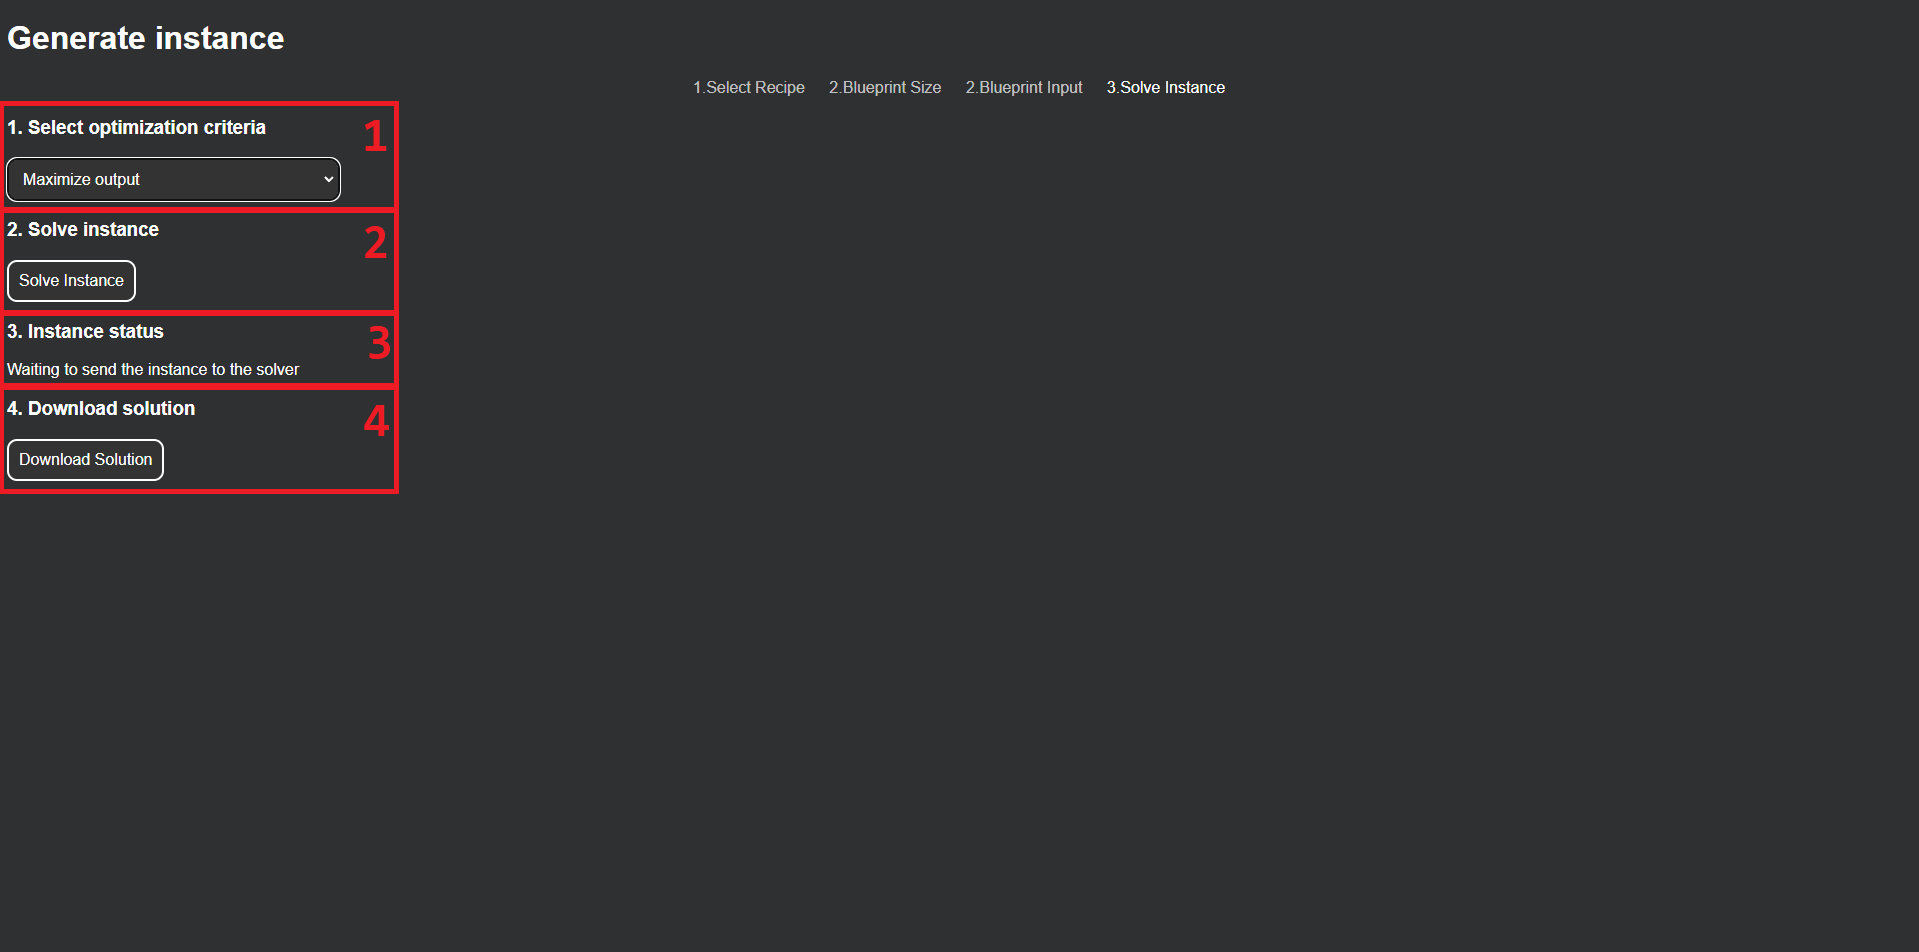
\includegraphics[width=1\linewidth]{Figures//captures_web/generate_instance_solving_web.PNG}
    \caption{Últim pas de la generació de la instància (1.Seleccionar l'objectiu d'optimització, 2.Botó per enviar la instància a resoldre, 3.Informació amb l'estat del procés de solving, 4.Botó per baixar el fitxer amb la solució a la instància)}
    \label{fig:generate_instance_solving}
\end{figure}


\subsection{Visualitzar instàncies}
La segona part del front end tracta del visualitzador d'instàncies, aquest té la seva pròpia pàgina HTML. La interacció, de manera similar a la selecció d'entrades i sortides del generador d'instàncies, es fa mitjançant un canvas el qual conté tota la part interactiva i s'encarrega de mostrar de manera visual tota la informació relativa a cada casella de la instància resolta.\\
A més també hi ha una part a l'HTML que mostra informació més detallada de la casella, el tipus d'objectes que transporta, quantitats... En cas que la casella seleccionada tracti d'un assemblador es mostra informació addicional com la recepta que produeix les quantitats d'entrada i sortida i les seves ràtios. Tot seguit algunes imatges de com està distribuïda la pàgina i com es mostren diferents informacions en funció de la instància (SAT, UNSAT) i les caselles seleccionades.

\begin{figure}[H]
    \centering
    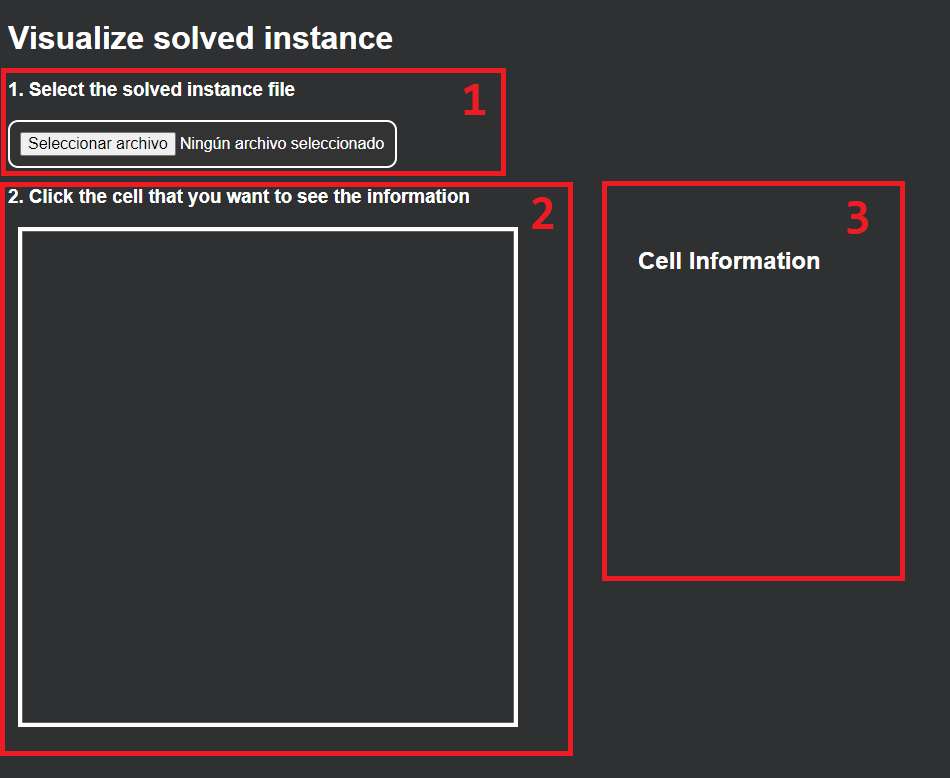
\includegraphics[width=1\linewidth]{Figures//captures_web/visualize_instance_basic.PNG}
    \caption{Distribució dels elements (1.Seleccionador d'instàncies resoltes, 2.Canvas on es mostra la informació de la instància, 3.Informació especifica de la casella seleccionada)}
    \label{fig:visualize_basic}
\end{figure}


\begin{figure}[H]
    \centering
    \begin{subfigure}{0.45\textwidth}
        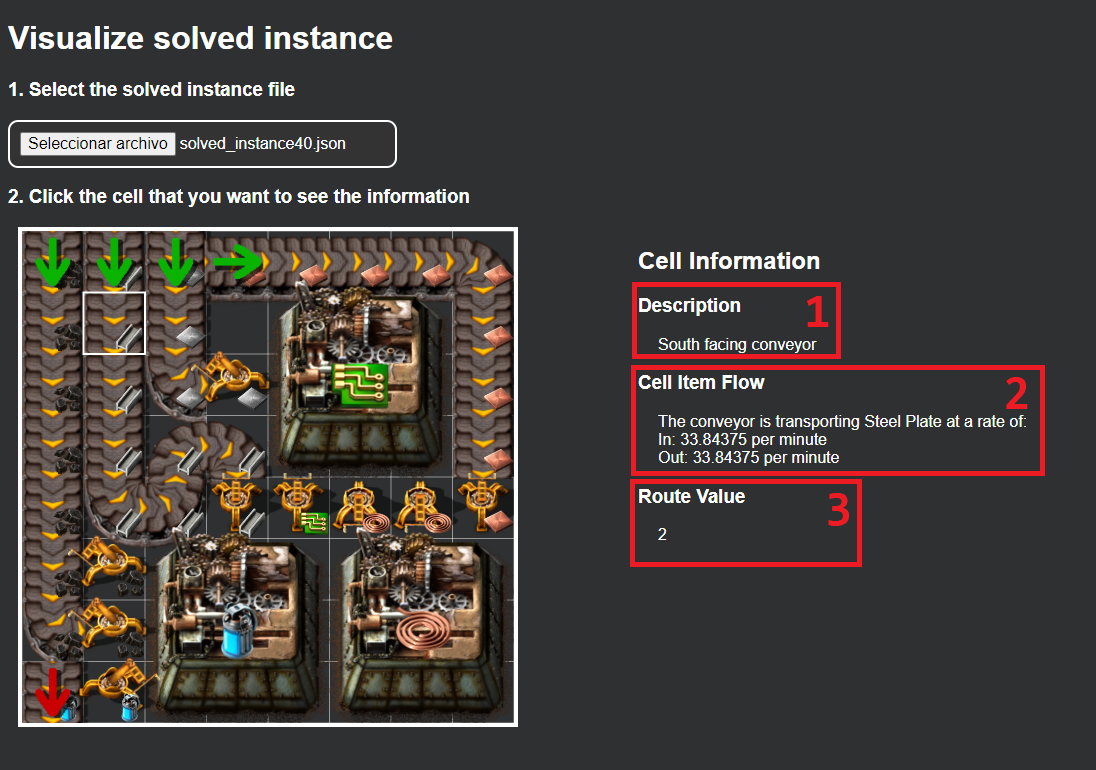
\includegraphics[width=\textwidth]{Figures/captures_web/visualize_instance_sat_conv.png}
        \caption{Informació d'una cinta (1.Breu descripció de la casella, 2.Quantitat d'objectes que entren i surten de la cinta, 3.Valor de ruta que té la cinta)}
    \end{subfigure}
    \hfill
    \begin{subfigure}{0.45\textwidth}
        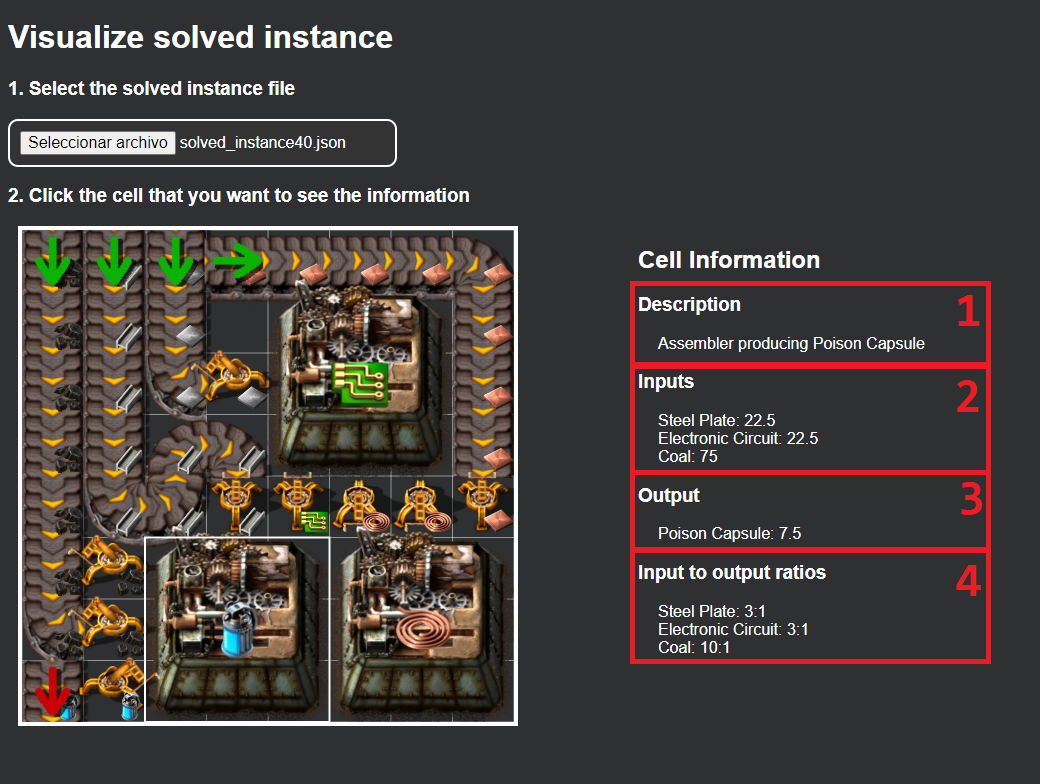
\includegraphics[width=\textwidth]{Figures/captures_web/visualize_instance_sat_ass.png}
        \caption{Informació d'un assemblador (1.Breu descripció de la casella, 2.Objectes i quantitats que entren a l'assemblador, 3.Objecte i quantitat que l'assemblador produeix, 4.Ràtios entre els objectes d'entrada i l'objecte produït)}
    \end{subfigure}
    \caption{Exemple de com es veu una instància resolta i la informació dels seus elements}
\end{figure}

\begin{figure}[H]
    \centering
    \begin{subfigure}{0.3\textwidth}
        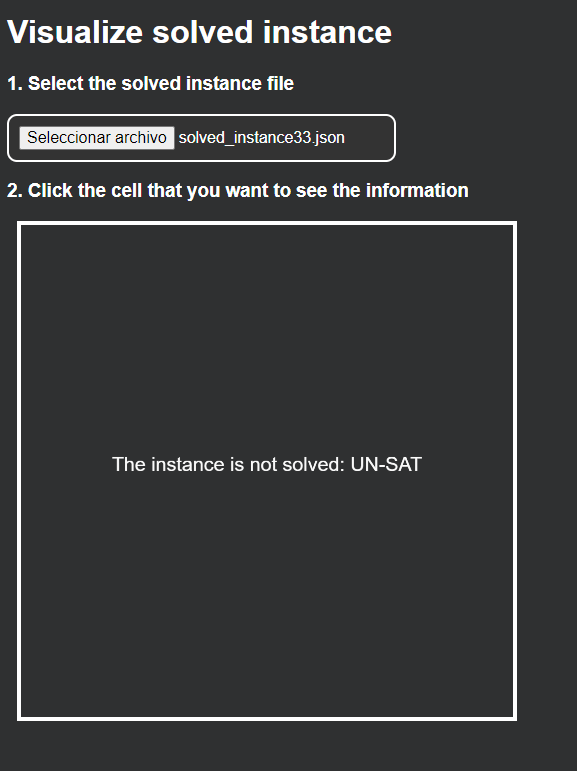
\includegraphics[width=\textwidth]{Figures/captures_web/visualize_instance_unsat.PNG}
        \caption{Instància sense solució}
    \end{subfigure}
    \hfill
    \begin{subfigure}{0.3\textwidth}
        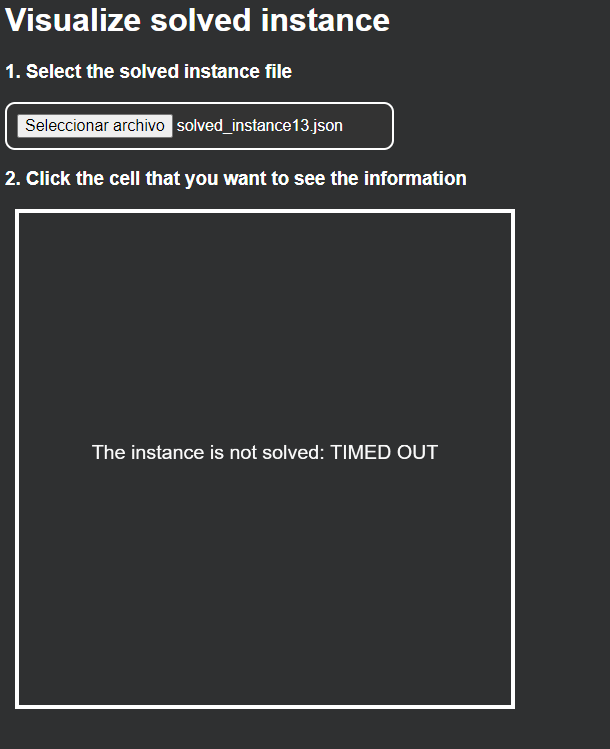
\includegraphics[width=\textwidth]{Figures/captures_web/visualize_instance_time_out.PNG}
        \caption{Instància no resolta}
    \end{subfigure}
    \hfill
    \begin{subfigure}{0.3\textwidth}
        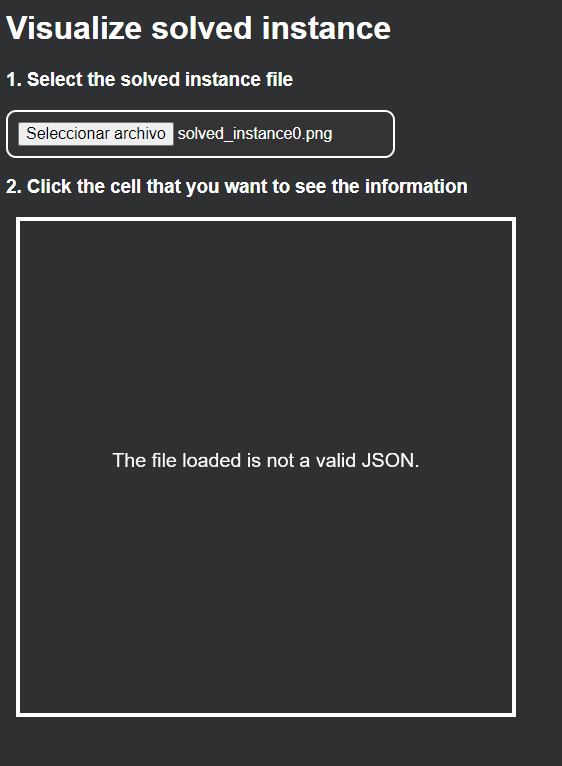
\includegraphics[width=\textwidth]{Figures/captures_web/visualize_instance_incorrect_file.PNG}
        \caption{Fitxer incorrecte}
    \end{subfigure}
    \caption{Exemples de com es capturen i mostren diferents errors}
\end{figure}


\section{Implementació de la pàgina web}
Com s'ha pogut veure a l'apartat anterior la pàgina es divideix en dos apartats principals, la generació i la visualització de les instàncies. Les dues parts, tot i complir funcionalitats diferents, comparteixen molts aspectes sobretot pel que fa a la part interactiva del canvas. Per això s'ha decidit usar el mecanisme d'herència de JavaScript per poder implementar funcionalitats comunes entre les dues parts i després implementar funcionalitats específiques per separat. A continuació l'explicació en detall de com s'ha fet el disseny de la part interactiva amb canvas i ús d'herència.

\subsection{Disseny del canvas interactiu}
El canvas és un element bàsic d'HTML que permet dibuixar imatges, formes geomètriques, text... Per aquest projecte s'ha decidit usar pel fet que no depèn d'altres llibreries i no afegeix més capes de complexitat al projecte.\\
Aquest element s'ha usat en dues parts de la web, a la generació d'instàncies, concretament a l'hora de seleccionar per quines caselles entren els materials i quines caselles són de sortida i per mostrar tots els elements de les instàncies resoltes.\\

Com hi ha moltes funcionalitats que són iguals tant al canvas de generació d'instàncies com el de visualització, s'ha optat per crear una classe abstracta \texttt{Blueprint}, que conté els atributs compartits com mida, casella seleccionada, la referència a l'element canvas HTML, nombre de files, nombre de columnes, informació de la graella... A més també implementa els mètodes encarregats de dibuixar la graella, detectar els clics a les caselles, actualitzar la informació d'una casella seleccionada... Finalment també obliga a les classes que hereten d'ella a implementar el mètode encarregat de reiniciar el canvas.

\begin{figure}[H]
    \centering
    \resizebox{\textwidth}{!}{
        \begin{tikzpicture}
            \begin{abstractclass}[text width=10cm]{Blueprint}{0,0}
                \attribute{- spriteCanvas : htmlObj}
                \attribute{- spriteContext : htmlObj}
                \attribute{- cursorCanvas : htmlObj}
                \attribute{- rows : int}
                \attribute{- columns : int}
                \attribute{- selectedCellX : int}
                \attribute{- selectedCellY : int}
                \attribute{- gridInformation : array}
                \attribute{- boundHandleCellClick : event}
                \operation[0]{+ resetBlueprint() : void}
                \operation{+ constructor()}
                \operation{- calculateGridSize(rows: int, cols: int) : void}
                \operation{- getCellCenter() : [int, int]}
                \operation{- handleCellClick(e : event) : void}
                \operation{- updateSelectedCell(e : event) : void}
                \operation{- drawGrid(rows : int, cols : int, color: string) : void}
                \operation{- formatItemName(name : string) : string}
                \operation{- removeAllEventListeners() : void}
            \end{abstractclass}
            
            \begin{class}[text width=8cm]{InputBlueprint}{-5, -12}
                \inherit{Blueprint}
                \attribute{- itemsList : list}
                \operation{+ resetGridInfo() : void}
                \operation{- itemSelectionHandler() : void}
                \operation{- isOutputHandler() : void}
                \operation{- sizeInputHandler() : void}
                \operation{- setItemsInUse(items : list) : void}
                \operation{- inputItems(item : string) : dict}
                \operation{- drawBlueprint() : void}
            \end{class}
            
            \begin{class}[text width=10cm]{SolvedBlueprint}{5, -12}
                \inherit{Blueprint}
                \attribute{- solvedInstance : dict}
                \attribute{- adjacentPos : dict}
                \attribute{- dirCoord : dict}
                \attribute{- oppositeDir : dict}
                \attribute{- spriteNames : array}
                \attribute{- sprites : dict}
                \operation{+ resetGridInfo() : void}
                \operation{+ draw() : void}
                \operation{- conveyorSprite(x : int, y : int) : string}
                \operation{- fetchSprite(spriteName : string) : void}
                \operation{- updateAssemblerInputOutput(x : int, y : int) : void}
                \operation{- conveyorRouteStatus(x : int, y : int) : string}
                \operation{- toFloat(number : string) : float}
            \end{class}
        \end{tikzpicture}
    }
    \caption{Diagrama de classes amb l'estructura seguida per implementar els canvas interactius}
    \label{fig:blueprint_class_diagram}
\end{figure}


Una part molt important del canvas interactiu és com emmagatzemar la informació de cada casella. Com hi ha diferents tipus de casella i cadascuna ha de guardar informació diferent i s'ha de representar gràficament al canvas de manera diferent, s'ha decidit guardar de la següent manera:

\subsubsection{Estructura de dades per guardar la informació de la graella}
Per guardar la informació de cada casella s'ha fet de manera similar a la classe \texttt{Blueprint}. S'ha creat una classe abstracta \texttt{Cell} que conté la informació que totes les caselles comparteixen i després s'han creat diferents classes que hereten d'aquesta i implementen els seus mètodes específics, d'aquesta manera es pot tenir una matriu, en aquest cas \texttt{gridInformation}, amb cel·les que parteixen de la mateixa classe pare i implementen el mateix mètode de maneres diferents, permetent així tenir un codi més net i genèric.\\
L'estructura de classes, atributs i mètodes queda de la següent manera:


\begin{figure}[H]
    \centering
    \rotatebox{90}{
        \scalebox{0.65}{
            \begin{tikzpicture}
                \begin{abstractclass}[text width=12cm]{Cell}{0,0}
                    \attribute{- x : float}
                    \attribute{- y : float}
                    \attribute{- type : string}
                    \operation[0]{+ updateCellInfo() : void}
                    \operation{+ constructor(x : float, y : float, type : string)}
                    \operation{+ draw(spr : image, canvas : htmlObj, rows : int, cols : int) : void}
                    \operation{+ drawItem(spr : image, canvas : htmlObj, cellSize : float) : void}
                    \operation{+ createInfoElement(title : string, value:string) : void}
                    \operation{+ drawSelectedOutline(canvas : htmlObj, rows : int, cols : int) : void}

                \end{abstractclass}
                
                \begin{class}[text width=12cm]{ConveyorCell}{-15, -10}
                    \inherit{Cell}
                    \attribute{- dir : string}
                    \attribute{- itemCarrying : string}
                    \attribute{- inputFlow : float}
                    \attribute{- outputFlow : float}
                    \attribute{- routeValue : int}
                    \attribute{- routeStatus : string}
                    \operation{+ constructor(dir : string, ic : string, if : float, of : float, rv : int, x : float, y : float, type : string)}
                    \operation{+ draw(spr : image, itemSpr: image, canvas : htmlObj, rows : int, cols : int) : void}
                    \operation{+ updateCellInfo() : void}
                \end{class}
                
                \begin{class}[text width=8cm]{InserterCell}{12, -10}
                    \inherit{Cell}
                    \operation{+ constructor(dir : string, ic : string, if : float, of : float, rv : int, x : float, y : float, type : string)}
                    \operation{+ draw(spr : image, itemSpr: image, canvas : htmlObj, rows : int, cols : int) : void}
                    \operation{+ updateCellInfo() : void}
                \end{class}

                \begin{class}[text width=12cm]{AssemblerCell}{0, -15}
                    \inherit{Cell}
                    \attribute{- itemProducing : string}
                    \attribute{- isDrawn : bool}
                    \attribute{- inputItems : dict}
                    \attribute{- outputItem : dict}
                    \operation{+ constructor(itemProducing : string, x : float, y : float)}
                    \operation{+ draw(spr : image, itemSpr: image, canvas : htmlObj, rows : int, cols : int) : void}
                    \operation{+ updateCellInfo() : void}
                    \operation{+ drawItem(spr : image, canvas : htmlObj, cellSize : float) : void}
                    \operation{- calculateRatios(input : dict, output : dict) : ratios : dict}
                    \operation{+ drawSelectedOutline(canvas : htmlObj, rows : int, columns : int) : void}
                    \operation{- createInfoElementWithDictionary(title : string, content : dict) : void}
                \end{class}

                \begin{class}[text width=6cm]{InputCell}{-4, -10}
                    \inherit{Cell}
                    \attribute{- itemCarrying : string}
                    \attribute{- isOutput : bool}
                    \operation{+ constructor(x : float, y : float)}
                    \operation{+ updateCellInfo() : void}
                \end{class}

                \begin{class}[text width=6cm]{EmptyCell}{4, -10}
                    \inherit{Cell}
                    \attribute{- description : string}
                    \operation{+ constructor(x : float, y : float)}
                    \operation{+ updateCellInfo() : void}
                \end{class}
            \end{tikzpicture}
        }
    }
    \caption{Diagrama de classes amb l'estructura de les diferents caselles}
    \label{fig:cell_class_diagram}
\end{figure}


Amb aquesta estructura cada casella s'encarrega de com ha de mostrar la seva informació a la web, com dibuixar-se correctament al canvas i com emmarcar-se per fer veure que ha sigut seleccionada.

\subsection{Alguns detalls interessants}
Al llarg de la implementació s'han hagut de prendre algunes decisions que són importants i s'han de mencionar.

\subsubsection{Demanar imatges al servidor}
Els canvas d'HTML dibuixen les imatges en ordre de crida de la funció \texttt{drawImage}, així que per obtenir el resultat correcte és molt important fer les crides de dibuixat en ordre, això pot semblar una ximpleria si el codi que sestà fent és concurrent, però en cas de les aplicacions web obtenir imatges es fa en paral·lel, ja que s'han de sol·licitar al servidor, fent que si no s'han carregat totes les imatges prèviament, aquestes es dibuixaran en ordre d'arribada fent que l'ordre de dibuixar inicial es perdi. Per arreglar aquest problema s'ha creat una funció que demana al servidor totes les imatges que la instància resolta necessita i aquestes es guarden en un diccionari que més tard es podrà consultar de manera completament síncrona.\\

\begin{lstlisting}[language=Java, caption=Fetch sprite]
    fetchSprite(spriteName){
        return new Promise((resolve, reject) => {
            let img = new Image();
            img.onload = () => resolve(img);
            img.onerror = reject;
            img.src = `/static/${spriteName}.png`;
        });
    }
\end{lstlisting}

Aquesta funció retorna una promesa d'aquesta manera des de fora, es pot fer un codi que fins que totes les promeses corresponents a cada imatge no s'hagin resolt, no s'executi cert codi, per exemple es pot fer el següent:

\begin{lstlisting}[language=Java, caption=Fetch all sprites]
    Promise.all(this.spriteNames.map(this.fetchSprite)).then(sprites => {
        this.sprites = Object.fromEntries(this.spriteNames.map((name, i) => [name, sprites[i]]));
           //Codi que s'executara despres de rebre totes les imatges
    });
\end{lstlisting}

Amb aquest tall de codi el que s'està fent és cridar la funció anterior per cada imatge guardada a la llista \texttt{spriteNames} i fins que no s'han rebut totes no es continua, assegurant així que si després es volen dibuixar les imatges aquestes no s'hagin d'anar a buscar.

\subsubsection{Evitar fer crides de dibuixat innecessàries}
Un altre detall és que si es vol modificar alguna part del que s'hagi dibuixat al canvas HTML, cal esborrar tot el que hi havia, modificar la part desitjada i tornar a dibuixar, això com es pot comprendre només és factible si hi ha moltes parts del canvas que s'estan canviant, però si només és un element no val la pena. Per això s'ha decidit que per emmarcar la casella seleccionada no es faci al mateix canvas on es dibuixen tots els elements sinó que millor crear un segon canvas, superposar-lo al canvas on es dibuixen tots els elements i així només s'ha d'esborrar i redibuixar el quadrat que emmarca les caselles. D'aquesta manera es redueix molt temps de dibuixat quan la majoria d'elements del canvas són estàtiques.\\

Per aconseguir l'efecte de superposició dels canvas s'ha fet el següent:

\begin{lstlisting}[language=html, caption=Declaració dels canvas]
    <div id="canvas-container">
        <canvas id="model-view" width="1000" height="1000">
            Your browser does not support the HTML canvas tag.
        </canvas>
        <canvas id="cursor-canvas" width="1000" height="1000">
            Your browser does not support the HTML canvas tag.
        </canvas>
    </div>
\end{lstlisting}

\begin{lstlisting}[language=html, caption=Estil dels canvas]
    #canvas-container > canvas {
        position:absolute;
        left:0;
        top:0;
    }
\end{lstlisting}

Amb aquesta declaració només cal administrar el comportament de cada canvas des de JavaScript per obtenir el comportament desitjat.







